%\begin{figure}[H]%[h!]
%  \begin{center}
%\centerline{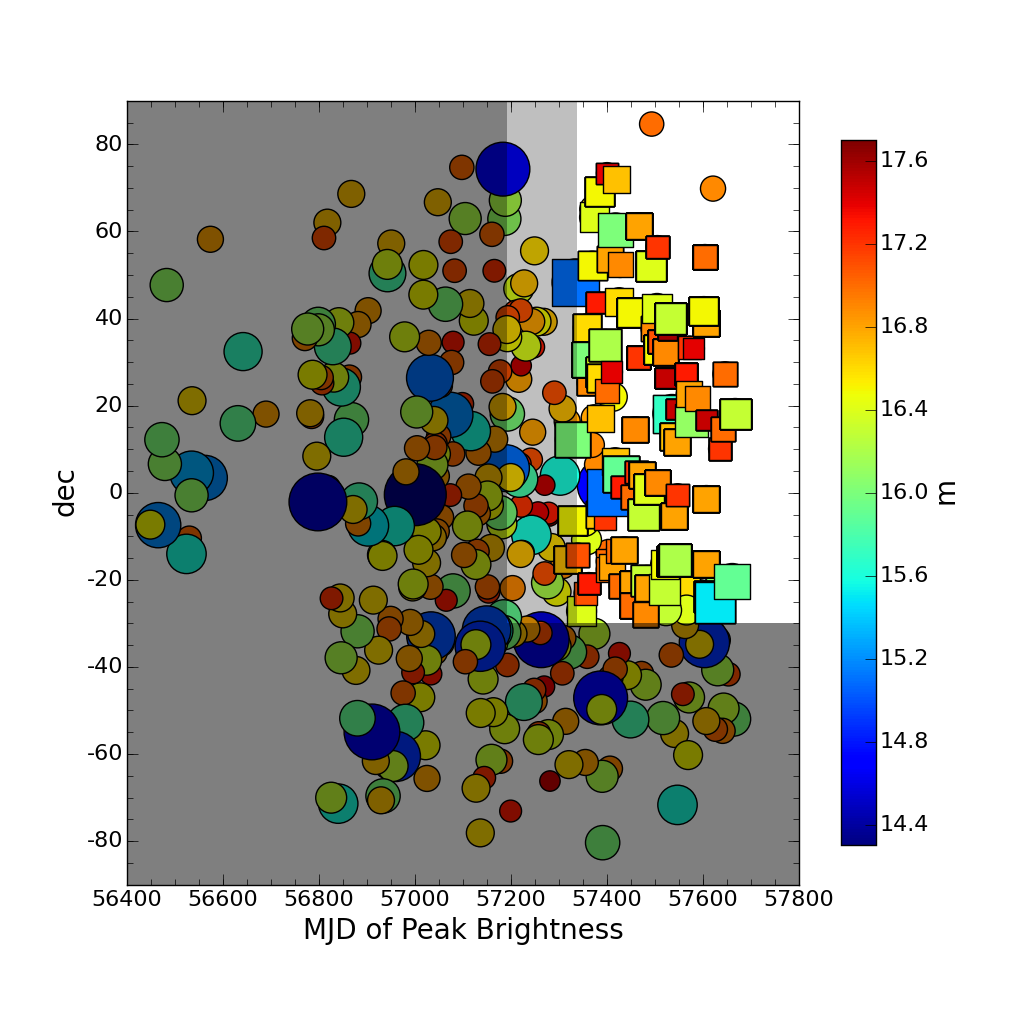
\includegraphics[width=3.35in]{figures/variations/invert_mag_shrink_9.png}}
%\caption{\it \small{{\bf cbar(shrink=0.9) choose this one or fullsize cbar} \label{fig:dec_mjd2}}}
%  \end{center}
%\end{figure}


{\bf Figures~\ref{fig:dec_mjd}~and~\ref{fig:var1} are exactly the same. All 4 plots in figure~\ref{fig:variations} show the same thing -- choose whichever represents the data in the best way}



\begin{figure*}
	\centering
	\begin{subfigure}{.5\textwidth}
	  \centering
	  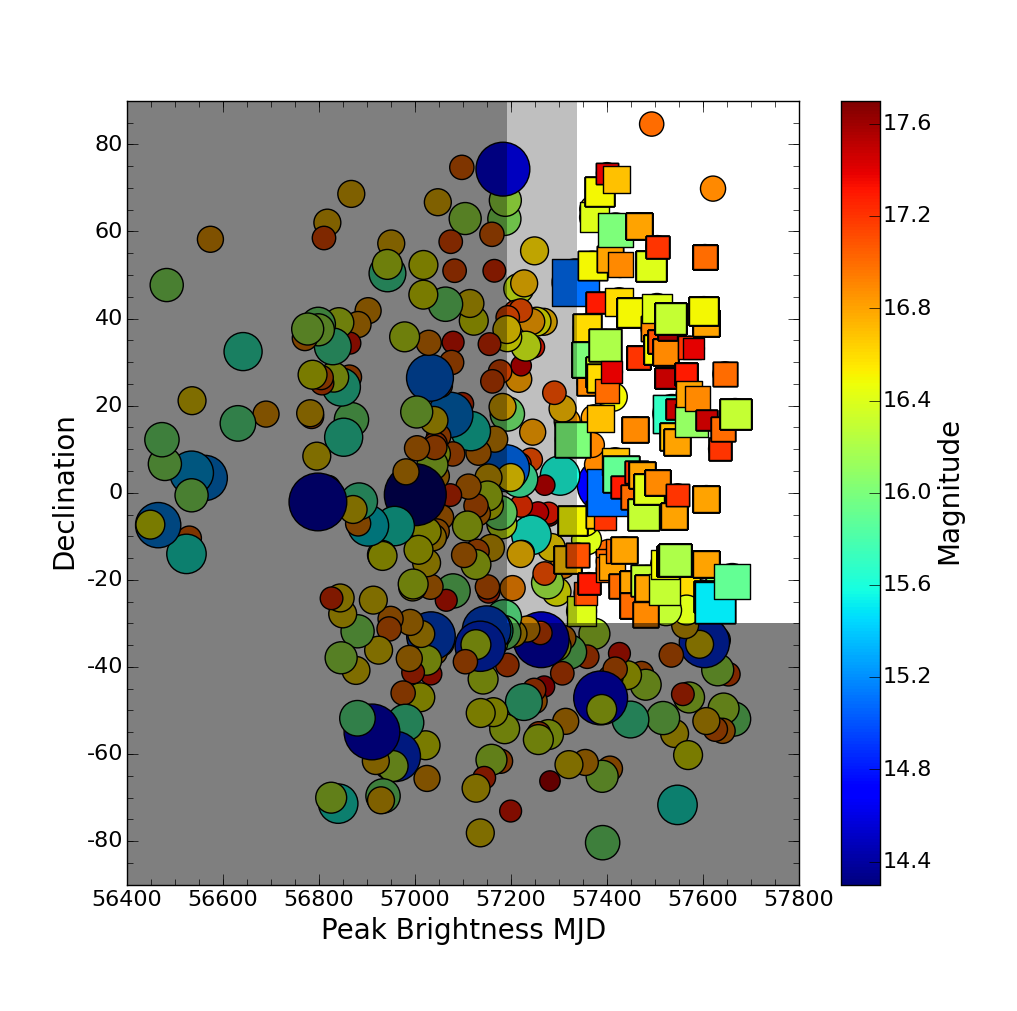
\includegraphics[width=1\linewidth]{figures/invert_mag.png}
		\caption{\it \small{ }}
		\label{fig:var1}
	\end{subfigure}%
	\begin{subfigure}{.5\textwidth}
	  \centering
			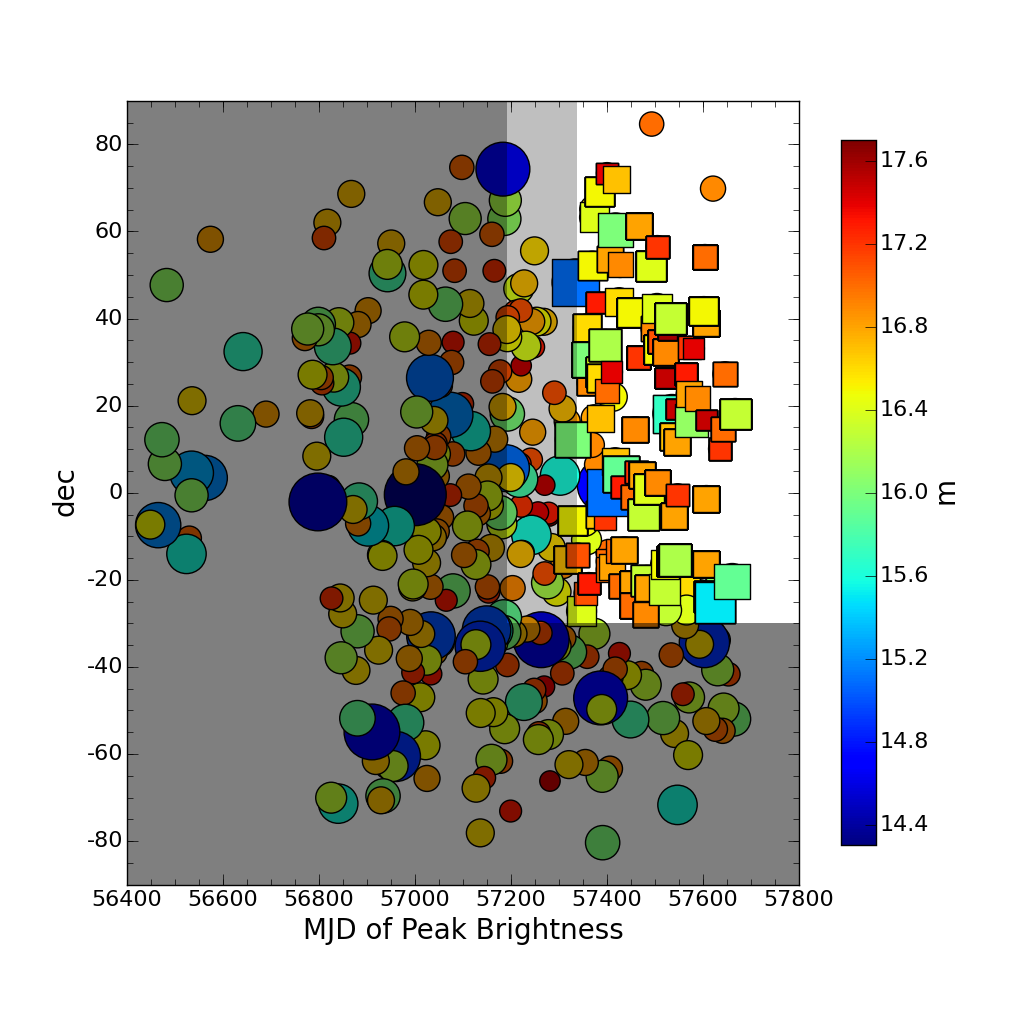
\includegraphics[width=1\linewidth]{figures/variations/invert_mag_shrink_9.png}
		\caption{\it \small{{\bf Same as (a) with cbar=0.9}}}
		\label{fig:var2}
	\end{subfigure}
	\begin{subfigure}{.5\textwidth}
	  \centering
	  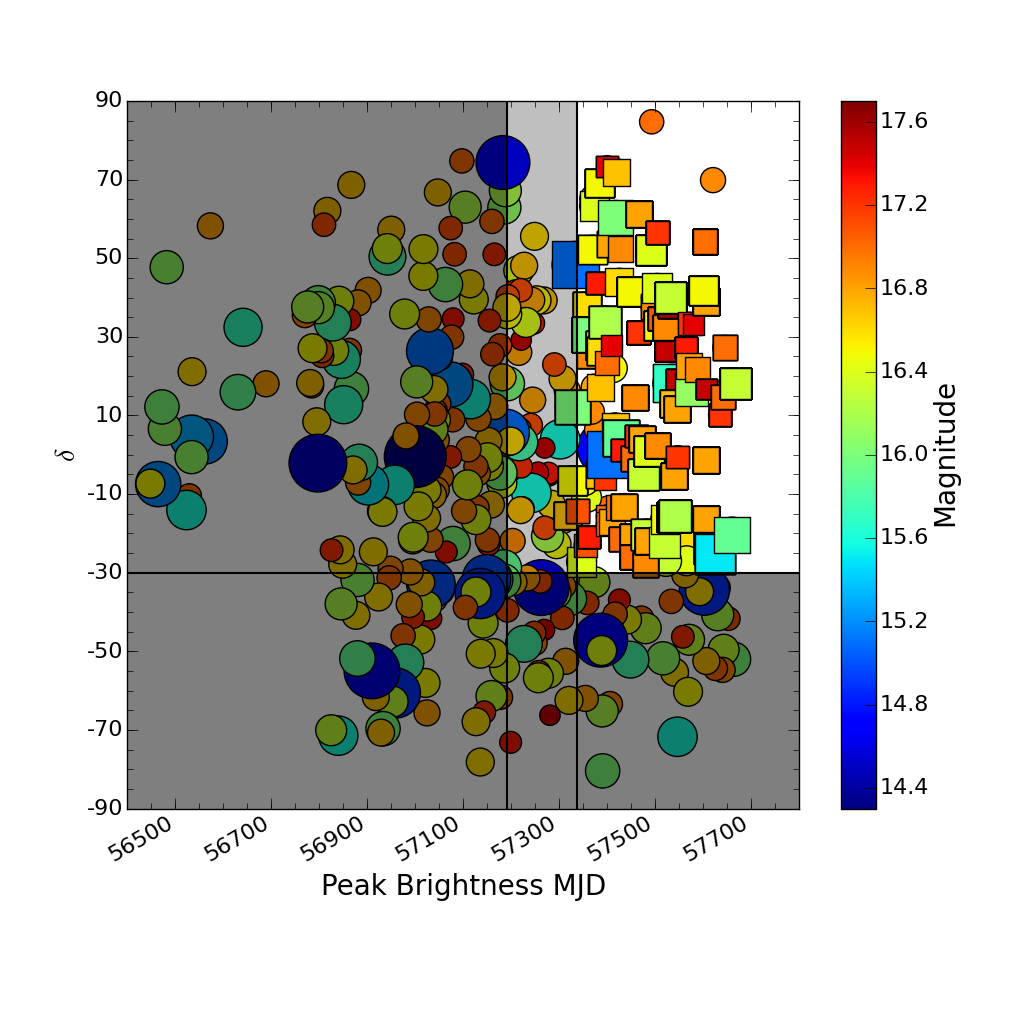
\includegraphics[width=1\linewidth]{figures/variations/shapes_invmag_fmt_vars.png}
		\caption{\it \small{{\bf cbar the same size as (a) but xtick labels are formatted differently. Differentiation between Grey regions has been made easier.}}}
		\label{fig:var3}
	\end{subfigure}%
	\begin{subfigure}{.5\textwidth}
	  \centering
			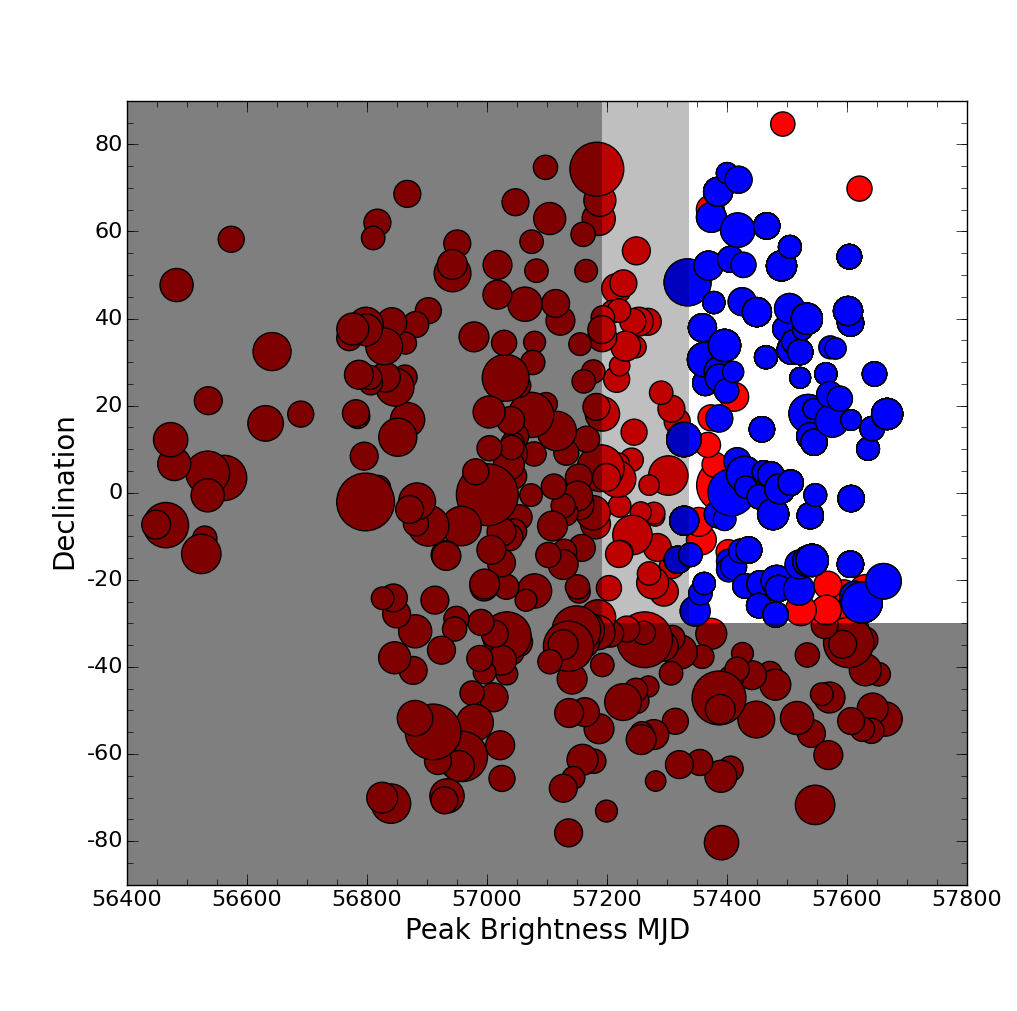
\includegraphics[width=1\linewidth]{figures/variations/mag_ps_not_color.png}
		\caption{\it \small{{\bf Here color is used to distinguish between SN that matched and those that didn't. Magnitude is still represented by point--size, with lower values having larger areas.}}}
		\label{fig:var4}
	\end{subfigure}
	\caption{\it \small{{\bf Panels (a), (b), (c), and (d) are all variations of the same plot. Slight variations in way labels; doesn't change content.}}}
	\label{fig:variations}
\end{figure*}



